\documentclass{article} % For LaTeX2e
\usepackage{iclr2019_conference,times}

% Optional math commands from https://github.com/goodfeli/dlbook_notation.
%%%%%% NEW MATH DEFINITIONS %%%%%

\usepackage{amsmath,amsfonts,bm}

% Mark sections of captions for referring to divisions of figures
\newcommand{\figleft}{{\em (Left)}}
\newcommand{\figcenter}{{\em (Center)}}
\newcommand{\figright}{{\em (Right)}}
\newcommand{\figtop}{{\em (Top)}}
\newcommand{\figbottom}{{\em (Bottom)}}
\newcommand{\captiona}{{\em (a)}}
\newcommand{\captionb}{{\em (b)}}
\newcommand{\captionc}{{\em (c)}}
\newcommand{\captiond}{{\em (d)}}

% Highlight a newly defined term
\newcommand{\newterm}[1]{{\bf #1}}


% Figure reference, lower-case.
\def\figref#1{figure~\ref{#1}}
% Figure reference, capital. For start of sentence
\def\Figref#1{Figure~\ref{#1}}
\def\twofigref#1#2{figures \ref{#1} and \ref{#2}}
\def\quadfigref#1#2#3#4{figures \ref{#1}, \ref{#2}, \ref{#3} and \ref{#4}}
% Section reference, lower-case.
\def\secref#1{section~\ref{#1}}
% Section reference, capital.
\def\Secref#1{Section~\ref{#1}}
% Reference to two sections.
\def\twosecrefs#1#2{sections \ref{#1} and \ref{#2}}
% Reference to three sections.
\def\secrefs#1#2#3{sections \ref{#1}, \ref{#2} and \ref{#3}}
% Reference to an equation, lower-case.
\def\eqref#1{equation~\ref{#1}}
% Reference to an equation, upper case
\def\Eqref#1{Equation~\ref{#1}}
% A raw reference to an equation---avoid using if possible
\def\plaineqref#1{\ref{#1}}
% Reference to a chapter, lower-case.
\def\chapref#1{chapter~\ref{#1}}
% Reference to an equation, upper case.
\def\Chapref#1{Chapter~\ref{#1}}
% Reference to a range of chapters
\def\rangechapref#1#2{chapters\ref{#1}--\ref{#2}}
% Reference to an algorithm, lower-case.
\def\algref#1{algorithm~\ref{#1}}
% Reference to an algorithm, upper case.
\def\Algref#1{Algorithm~\ref{#1}}
\def\twoalgref#1#2{algorithms \ref{#1} and \ref{#2}}
\def\Twoalgref#1#2{Algorithms \ref{#1} and \ref{#2}}
% Reference to a part, lower case
\def\partref#1{part~\ref{#1}}
% Reference to a part, upper case
\def\Partref#1{Part~\ref{#1}}
\def\twopartref#1#2{parts \ref{#1} and \ref{#2}}

\def\ceil#1{\lceil #1 \rceil}
\def\floor#1{\lfloor #1 \rfloor}
\def\1{\bm{1}}
\newcommand{\train}{\mathcal{D}}
\newcommand{\valid}{\mathcal{D_{\mathrm{valid}}}}
\newcommand{\test}{\mathcal{D_{\mathrm{test}}}}

\def\eps{{\epsilon}}


% Random variables
\def\reta{{\textnormal{$\eta$}}}
\def\ra{{\textnormal{a}}}
\def\rb{{\textnormal{b}}}
\def\rc{{\textnormal{c}}}
\def\rd{{\textnormal{d}}}
\def\re{{\textnormal{e}}}
\def\rf{{\textnormal{f}}}
\def\rg{{\textnormal{g}}}
\def\rh{{\textnormal{h}}}
\def\ri{{\textnormal{i}}}
\def\rj{{\textnormal{j}}}
\def\rk{{\textnormal{k}}}
\def\rl{{\textnormal{l}}}
% rm is already a command, just don't name any random variables m
\def\rn{{\textnormal{n}}}
\def\ro{{\textnormal{o}}}
\def\rp{{\textnormal{p}}}
\def\rq{{\textnormal{q}}}
\def\rr{{\textnormal{r}}}
\def\rs{{\textnormal{s}}}
\def\rt{{\textnormal{t}}}
\def\ru{{\textnormal{u}}}
\def\rv{{\textnormal{v}}}
\def\rw{{\textnormal{w}}}
\def\rx{{\textnormal{x}}}
\def\ry{{\textnormal{y}}}
\def\rz{{\textnormal{z}}}

% Random vectors
\def\rvepsilon{{\mathbf{\epsilon}}}
\def\rvtheta{{\mathbf{\theta}}}
\def\rva{{\mathbf{a}}}
\def\rvb{{\mathbf{b}}}
\def\rvc{{\mathbf{c}}}
\def\rvd{{\mathbf{d}}}
\def\rve{{\mathbf{e}}}
\def\rvf{{\mathbf{f}}}
\def\rvg{{\mathbf{g}}}
\def\rvh{{\mathbf{h}}}
\def\rvu{{\mathbf{i}}}
\def\rvj{{\mathbf{j}}}
\def\rvk{{\mathbf{k}}}
\def\rvl{{\mathbf{l}}}
\def\rvm{{\mathbf{m}}}
\def\rvn{{\mathbf{n}}}
\def\rvo{{\mathbf{o}}}
\def\rvp{{\mathbf{p}}}
\def\rvq{{\mathbf{q}}}
\def\rvr{{\mathbf{r}}}
\def\rvs{{\mathbf{s}}}
\def\rvt{{\mathbf{t}}}
\def\rvu{{\mathbf{u}}}
\def\rvv{{\mathbf{v}}}
\def\rvw{{\mathbf{w}}}
\def\rvx{{\mathbf{x}}}
\def\rvy{{\mathbf{y}}}
\def\rvz{{\mathbf{z}}}

% Elements of random vectors
\def\erva{{\textnormal{a}}}
\def\ervb{{\textnormal{b}}}
\def\ervc{{\textnormal{c}}}
\def\ervd{{\textnormal{d}}}
\def\erve{{\textnormal{e}}}
\def\ervf{{\textnormal{f}}}
\def\ervg{{\textnormal{g}}}
\def\ervh{{\textnormal{h}}}
\def\ervi{{\textnormal{i}}}
\def\ervj{{\textnormal{j}}}
\def\ervk{{\textnormal{k}}}
\def\ervl{{\textnormal{l}}}
\def\ervm{{\textnormal{m}}}
\def\ervn{{\textnormal{n}}}
\def\ervo{{\textnormal{o}}}
\def\ervp{{\textnormal{p}}}
\def\ervq{{\textnormal{q}}}
\def\ervr{{\textnormal{r}}}
\def\ervs{{\textnormal{s}}}
\def\ervt{{\textnormal{t}}}
\def\ervu{{\textnormal{u}}}
\def\ervv{{\textnormal{v}}}
\def\ervw{{\textnormal{w}}}
\def\ervx{{\textnormal{x}}}
\def\ervy{{\textnormal{y}}}
\def\ervz{{\textnormal{z}}}

% Random matrices
\def\rmA{{\mathbf{A}}}
\def\rmB{{\mathbf{B}}}
\def\rmC{{\mathbf{C}}}
\def\rmD{{\mathbf{D}}}
\def\rmE{{\mathbf{E}}}
\def\rmF{{\mathbf{F}}}
\def\rmG{{\mathbf{G}}}
\def\rmH{{\mathbf{H}}}
\def\rmI{{\mathbf{I}}}
\def\rmJ{{\mathbf{J}}}
\def\rmK{{\mathbf{K}}}
\def\rmL{{\mathbf{L}}}
\def\rmM{{\mathbf{M}}}
\def\rmN{{\mathbf{N}}}
\def\rmO{{\mathbf{O}}}
\def\rmP{{\mathbf{P}}}
\def\rmQ{{\mathbf{Q}}}
\def\rmR{{\mathbf{R}}}
\def\rmS{{\mathbf{S}}}
\def\rmT{{\mathbf{T}}}
\def\rmU{{\mathbf{U}}}
\def\rmV{{\mathbf{V}}}
\def\rmW{{\mathbf{W}}}
\def\rmX{{\mathbf{X}}}
\def\rmY{{\mathbf{Y}}}
\def\rmZ{{\mathbf{Z}}}

% Elements of random matrices
\def\ermA{{\textnormal{A}}}
\def\ermB{{\textnormal{B}}}
\def\ermC{{\textnormal{C}}}
\def\ermD{{\textnormal{D}}}
\def\ermE{{\textnormal{E}}}
\def\ermF{{\textnormal{F}}}
\def\ermG{{\textnormal{G}}}
\def\ermH{{\textnormal{H}}}
\def\ermI{{\textnormal{I}}}
\def\ermJ{{\textnormal{J}}}
\def\ermK{{\textnormal{K}}}
\def\ermL{{\textnormal{L}}}
\def\ermM{{\textnormal{M}}}
\def\ermN{{\textnormal{N}}}
\def\ermO{{\textnormal{O}}}
\def\ermP{{\textnormal{P}}}
\def\ermQ{{\textnormal{Q}}}
\def\ermR{{\textnormal{R}}}
\def\ermS{{\textnormal{S}}}
\def\ermT{{\textnormal{T}}}
\def\ermU{{\textnormal{U}}}
\def\ermV{{\textnormal{V}}}
\def\ermW{{\textnormal{W}}}
\def\ermX{{\textnormal{X}}}
\def\ermY{{\textnormal{Y}}}
\def\ermZ{{\textnormal{Z}}}

% Vectors
\def\vzero{{\bm{0}}}
\def\vone{{\bm{1}}}
\def\vmu{{\bm{\mu}}}
\def\vtheta{{\bm{\theta}}}
\def\va{{\bm{a}}}
\def\vb{{\bm{b}}}
\def\vc{{\bm{c}}}
\def\vd{{\bm{d}}}
\def\ve{{\bm{e}}}
\def\vf{{\bm{f}}}
\def\vg{{\bm{g}}}
\def\vh{{\bm{h}}}
\def\vi{{\bm{i}}}
\def\vj{{\bm{j}}}
\def\vk{{\bm{k}}}
\def\vl{{\bm{l}}}
\def\vm{{\bm{m}}}
\def\vn{{\bm{n}}}
\def\vo{{\bm{o}}}
\def\vp{{\bm{p}}}
\def\vq{{\bm{q}}}
\def\vr{{\bm{r}}}
\def\vs{{\bm{s}}}
\def\vt{{\bm{t}}}
\def\vu{{\bm{u}}}
\def\vv{{\bm{v}}}
\def\vw{{\bm{w}}}
\def\vx{{\bm{x}}}
\def\vy{{\bm{y}}}
\def\vz{{\bm{z}}}

% Elements of vectors
\def\evalpha{{\alpha}}
\def\evbeta{{\beta}}
\def\evepsilon{{\epsilon}}
\def\evlambda{{\lambda}}
\def\evomega{{\omega}}
\def\evmu{{\mu}}
\def\evpsi{{\psi}}
\def\evsigma{{\sigma}}
\def\evtheta{{\theta}}
\def\eva{{a}}
\def\evb{{b}}
\def\evc{{c}}
\def\evd{{d}}
\def\eve{{e}}
\def\evf{{f}}
\def\evg{{g}}
\def\evh{{h}}
\def\evi{{i}}
\def\evj{{j}}
\def\evk{{k}}
\def\evl{{l}}
\def\evm{{m}}
\def\evn{{n}}
\def\evo{{o}}
\def\evp{{p}}
\def\evq{{q}}
\def\evr{{r}}
\def\evs{{s}}
\def\evt{{t}}
\def\evu{{u}}
\def\evv{{v}}
\def\evw{{w}}
\def\evx{{x}}
\def\evy{{y}}
\def\evz{{z}}

% Matrix
\def\mA{{\bm{A}}}
\def\mB{{\bm{B}}}
\def\mC{{\bm{C}}}
\def\mD{{\bm{D}}}
\def\mE{{\bm{E}}}
\def\mF{{\bm{F}}}
\def\mG{{\bm{G}}}
\def\mH{{\bm{H}}}
\def\mI{{\bm{I}}}
\def\mJ{{\bm{J}}}
\def\mK{{\bm{K}}}
\def\mL{{\bm{L}}}
\def\mM{{\bm{M}}}
\def\mN{{\bm{N}}}
\def\mO{{\bm{O}}}
\def\mP{{\bm{P}}}
\def\mQ{{\bm{Q}}}
\def\mR{{\bm{R}}}
\def\mS{{\bm{S}}}
\def\mT{{\bm{T}}}
\def\mU{{\bm{U}}}
\def\mV{{\bm{V}}}
\def\mW{{\bm{W}}}
\def\mX{{\bm{X}}}
\def\mY{{\bm{Y}}}
\def\mZ{{\bm{Z}}}
\def\mBeta{{\bm{\beta}}}
\def\mPhi{{\bm{\Phi}}}
\def\mLambda{{\bm{\Lambda}}}
\def\mSigma{{\bm{\Sigma}}}

% Tensor
\DeclareMathAlphabet{\mathsfit}{\encodingdefault}{\sfdefault}{m}{sl}
\SetMathAlphabet{\mathsfit}{bold}{\encodingdefault}{\sfdefault}{bx}{n}
\newcommand{\tens}[1]{\bm{\mathsfit{#1}}}
\def\tA{{\tens{A}}}
\def\tB{{\tens{B}}}
\def\tC{{\tens{C}}}
\def\tD{{\tens{D}}}
\def\tE{{\tens{E}}}
\def\tF{{\tens{F}}}
\def\tG{{\tens{G}}}
\def\tH{{\tens{H}}}
\def\tI{{\tens{I}}}
\def\tJ{{\tens{J}}}
\def\tK{{\tens{K}}}
\def\tL{{\tens{L}}}
\def\tM{{\tens{M}}}
\def\tN{{\tens{N}}}
\def\tO{{\tens{O}}}
\def\tP{{\tens{P}}}
\def\tQ{{\tens{Q}}}
\def\tR{{\tens{R}}}
\def\tS{{\tens{S}}}
\def\tT{{\tens{T}}}
\def\tU{{\tens{U}}}
\def\tV{{\tens{V}}}
\def\tW{{\tens{W}}}
\def\tX{{\tens{X}}}
\def\tY{{\tens{Y}}}
\def\tZ{{\tens{Z}}}


% Graph
\def\gA{{\mathcal{A}}}
\def\gB{{\mathcal{B}}}
\def\gC{{\mathcal{C}}}
\def\gD{{\mathcal{D}}}
\def\gE{{\mathcal{E}}}
\def\gF{{\mathcal{F}}}
\def\gG{{\mathcal{G}}}
\def\gH{{\mathcal{H}}}
\def\gI{{\mathcal{I}}}
\def\gJ{{\mathcal{J}}}
\def\gK{{\mathcal{K}}}
\def\gL{{\mathcal{L}}}
\def\gM{{\mathcal{M}}}
\def\gN{{\mathcal{N}}}
\def\gO{{\mathcal{O}}}
\def\gP{{\mathcal{P}}}
\def\gQ{{\mathcal{Q}}}
\def\gR{{\mathcal{R}}}
\def\gS{{\mathcal{S}}}
\def\gT{{\mathcal{T}}}
\def\gU{{\mathcal{U}}}
\def\gV{{\mathcal{V}}}
\def\gW{{\mathcal{W}}}
\def\gX{{\mathcal{X}}}
\def\gY{{\mathcal{Y}}}
\def\gZ{{\mathcal{Z}}}

% Sets
\def\sA{{\mathbb{A}}}
\def\sB{{\mathbb{B}}}
\def\sC{{\mathbb{C}}}
\def\sD{{\mathbb{D}}}
% Don't use a set called E, because this would be the same as our symbol
% for expectation.
\def\sF{{\mathbb{F}}}
\def\sG{{\mathbb{G}}}
\def\sH{{\mathbb{H}}}
\def\sI{{\mathbb{I}}}
\def\sJ{{\mathbb{J}}}
\def\sK{{\mathbb{K}}}
\def\sL{{\mathbb{L}}}
\def\sM{{\mathbb{M}}}
\def\sN{{\mathbb{N}}}
\def\sO{{\mathbb{O}}}
\def\sP{{\mathbb{P}}}
\def\sQ{{\mathbb{Q}}}
\def\sR{{\mathbb{R}}}
\def\sS{{\mathbb{S}}}
\def\sT{{\mathbb{T}}}
\def\sU{{\mathbb{U}}}
\def\sV{{\mathbb{V}}}
\def\sW{{\mathbb{W}}}
\def\sX{{\mathbb{X}}}
\def\sY{{\mathbb{Y}}}
\def\sZ{{\mathbb{Z}}}

% Entries of a matrix
\def\emLambda{{\Lambda}}
\def\emA{{A}}
\def\emB{{B}}
\def\emC{{C}}
\def\emD{{D}}
\def\emE{{E}}
\def\emF{{F}}
\def\emG{{G}}
\def\emH{{H}}
\def\emI{{I}}
\def\emJ{{J}}
\def\emK{{K}}
\def\emL{{L}}
\def\emM{{M}}
\def\emN{{N}}
\def\emO{{O}}
\def\emP{{P}}
\def\emQ{{Q}}
\def\emR{{R}}
\def\emS{{S}}
\def\emT{{T}}
\def\emU{{U}}
\def\emV{{V}}
\def\emW{{W}}
\def\emX{{X}}
\def\emY{{Y}}
\def\emZ{{Z}}
\def\emSigma{{\Sigma}}

% entries of a tensor
% Same font as tensor, without \bm wrapper
\newcommand{\etens}[1]{\mathsfit{#1}}
\def\etLambda{{\etens{\Lambda}}}
\def\etA{{\etens{A}}}
\def\etB{{\etens{B}}}
\def\etC{{\etens{C}}}
\def\etD{{\etens{D}}}
\def\etE{{\etens{E}}}
\def\etF{{\etens{F}}}
\def\etG{{\etens{G}}}
\def\etH{{\etens{H}}}
\def\etI{{\etens{I}}}
\def\etJ{{\etens{J}}}
\def\etK{{\etens{K}}}
\def\etL{{\etens{L}}}
\def\etM{{\etens{M}}}
\def\etN{{\etens{N}}}
\def\etO{{\etens{O}}}
\def\etP{{\etens{P}}}
\def\etQ{{\etens{Q}}}
\def\etR{{\etens{R}}}
\def\etS{{\etens{S}}}
\def\etT{{\etens{T}}}
\def\etU{{\etens{U}}}
\def\etV{{\etens{V}}}
\def\etW{{\etens{W}}}
\def\etX{{\etens{X}}}
\def\etY{{\etens{Y}}}
\def\etZ{{\etens{Z}}}

% The true underlying data generating distribution
\newcommand{\pdata}{p_{\rm{data}}}
% The empirical distribution defined by the training set
\newcommand{\ptrain}{\hat{p}_{\rm{data}}}
\newcommand{\Ptrain}{\hat{P}_{\rm{data}}}
% The model distribution
\newcommand{\pmodel}{p_{\rm{model}}}
\newcommand{\Pmodel}{P_{\rm{model}}}
\newcommand{\ptildemodel}{\tilde{p}_{\rm{model}}}
% Stochastic autoencoder distributions
\newcommand{\pencode}{p_{\rm{encoder}}}
\newcommand{\pdecode}{p_{\rm{decoder}}}
\newcommand{\precons}{p_{\rm{reconstruct}}}

\newcommand{\laplace}{\mathrm{Laplace}} % Laplace distribution

\newcommand{\E}{\mathbb{E}}
\newcommand{\Ls}{\mathcal{L}}
\newcommand{\R}{\mathbb{R}}
\newcommand{\emp}{\tilde{p}}
\newcommand{\lr}{\alpha}
\newcommand{\reg}{\lambda}
\newcommand{\rect}{\mathrm{rectifier}}
\newcommand{\softmax}{\mathrm{softmax}}
\newcommand{\sigmoid}{\sigma}
\newcommand{\softplus}{\zeta}
\newcommand{\KL}{D_{\mathrm{KL}}}
\newcommand{\Var}{\mathrm{Var}}
\newcommand{\standarderror}{\mathrm{SE}}
\newcommand{\Cov}{\mathrm{Cov}}
% Wolfram Mathworld says $L^2$ is for function spaces and $\ell^2$ is for vectors
% But then they seem to use $L^2$ for vectors throughout the site, and so does
% wikipedia.
\newcommand{\normlzero}{L^0}
\newcommand{\normlone}{L^1}
\newcommand{\normltwo}{L^2}
\newcommand{\normlp}{L^p}
\newcommand{\normmax}{L^\infty}

\newcommand{\parents}{Pa} % See usage in notation.tex. Chosen to match Daphne's book.

\DeclareMathOperator*{\argmax}{arg\,max}
\DeclareMathOperator*{\argmin}{arg\,min}

\DeclareMathOperator{\sign}{sign}
\DeclareMathOperator{\Tr}{Tr}
\let\ab\allowbreak



\usepackage[utf8]{inputenc} % allow utf-8 input
\usepackage[T1]{fontenc}    % use 8-bit T1 fonts
\usepackage{hyperref}       % hyperlinks
\usepackage{url}            % simple URL typesetting
\usepackage{booktabs}       % professional-quality tables
\usepackage{amsfonts}       % blackboard math symbols
\usepackage{nicefrac}       % compact symbols for 1/2, etc.
\usepackage{microtype}      % microtypography

\usepackage{hyperref}

\usepackage{amssymb}
\usepackage{amsmath}

% For citations
%\usepackage[numbers, sort&compress]{natbib}
%\usepackage[numbers]{natbib}
%\usepackage{natbib}

% For figures
\usepackage{graphicx} % more modern
\usepackage{wrapfig}
%\usepackage{epsfig} % less modern
%\usepackage{subfigure} 
\usepackage{subcaption} 
\usepackage{multirow}
\usepackage{adjustbox}

\usepackage{listings}
\usepackage{textcomp}

% For assumptions
\usepackage{amsthm,amssymb,amsopn}
\newtheorem{assumption}{Assumption}
\newtheorem{define}{Definition}
\newtheorem{thm}{Theorem}
\newtheorem{lem}{Lemma}
\newtheorem{coro}{Corollary}
\newtheorem{condition}{Condition}
\usepackage{xspace}
\usepackage{bm}

% For algorithms
\usepackage{algorithm}
\usepackage{algorithmic}
\renewcommand{\algorithmiccomment}[1]{~~~~\textcolor{gray}{$\triangleright$\textit{#1}}}
\renewcommand{\algorithmicrequire}{\textbf{Input:}}
\renewcommand{\algorithmicensure}{\textbf{Output:}}
\makeatletter
\makeatletter
\newcommand*{\da@rightarrow}{\mathchar"0\hexnumber@\symAMSa 4B }
\newcommand*{\da@leftarrow}{\mathchar"0\hexnumber@\symAMSa 4C }
\newcommand*{\xdashrightarrow}[2][]{%
  \mathrel{%
    \mathpalette{\da@xarrow{#1}{#2}{}\da@rightarrow{\,}{}}{}%
  }%
}
\newcommand{\xdashleftarrow}[2][]{%
  \mathrel{%
    \mathpalette{\da@xarrow{#1}{#2}\da@leftarrow{}{}{\,}}{}%
  }%
}
\newcommand*{\da@xarrow}[7]{%
  % #1: below
  % #2: above
  % #3: arrow left
  % #4: arrow right
  % #5: space left 
  % #6: space right
  % #7: math style 
  \sbox0{$\ifx#7\scriptstyle\scriptscriptstyle\else\scriptstyle\fi#5#1#6\m@th$}%
  \sbox2{$\ifx#7\scriptstyle\scriptscriptstyle\else\scriptstyle\fi#5#2#6\m@th$}%
  \sbox4{$#7\dabar@\m@th$}%
  \dimen@=\wd0 %
  \ifdim\wd2 >\dimen@
    \dimen@=\wd2 %   
  \fi
  \count@=2 %
  \def\da@bars{\dabar@\dabar@}%
  \@whiledim\count@\wd4<\dimen@\do{%
    \advance\count@\@ne
    \expandafter\def\expandafter\da@bars\expandafter{%
      \da@bars
      \dabar@ 
    }%
  }%  
  \mathrel{#3}%
  \mathrel{%   
    \mathop{\da@bars}\limits
    \ifx\\#1\\%
    \else
      _{\copy0}%
    \fi
    \ifx\\#2\\%
    \else
      ^{\copy2}%
    \fi
  }%   
  \mathrel{#4}%
}
\makeatother

% for striking out.
\usepackage[normalem]{ulem}


\title{Predicting Electron Paths}

% The \author macro works with any number of authors. There are two
% commands used to separate the names and addresses of multiple
% authors: \And and \AND.
%
% Using \And between authors leaves it to LaTeX to determine where to
% break the lines. Using \AND forces a line break at that point. So,
% if LaTeX puts 3 of 4 authors names on the first line, and the last
% on the second line, try using \AND instead of \And before the third
% author name.




\author{John Bradshaw \\ 
University of Cambridge \\
Max Planck Institute, T\"ubingen 
\\
\texttt{jab255@cam.ac.uk}
\And
Matt J. Kusner \\
Alan Turing Institute \\
University of Warwick 
\\
\texttt{mkusner@turing.ac.uk}
\And
Brooks Paige \\
Alan Turing Institute \\
University of Cambridge 
\\
\texttt{bpaige@turing.ac.uk}
\AND
Marwin H. S. Segler \\
BenevolentAI \\
\texttt{marwin.segler@benevolent.ai}
\And
Jos\'e Miguel Hern\'andez-Lobato \\
University of Cambridge \\
Alan Turing Institute \\
\texttt{jmh233@cam.ac.uk}
}


\newcommand{\xb}{\mathbf{x}}
\newcommand{\Xc}{\mathcal{X}}
\newcommand{\Zc}{{\mathcal{Z}}}
\newcommand{\Mc}{{\mathcal{M}}}
\newcommand{\Bc}{{\mathcal{B}}}
\newcommand{\Ac}{{\mathcal{A}}}
\newcommand{\Pc}{{\mathcal{P}}}
\newcommand{\bb}{{\mathbf{b}}}
\newcommand{\ab}{{\mathbf{a}}}
\newcommand{\mb}{{\mathbf{m}}}
\newcommand{\Mb}{{\mathbf{M}}}
\newcommand{\Pb}{{\mathbf{P}}}
\newcommand{\Hb}{{\mathbf{H}}}
\newcommand{\Ab}{{\mathbf{A}}}
\newcommand{\Rc}{{\mathcal{R}}}
\newcommand{\delb}{{\boldmath{\delta}}}


%
\newcommand{\nodeEmbeddings}[1]{\Hb_{#1}}
\newcommand{\graphEmbeddings}{\mathbf{h_g}}
%\newcommand{\graph}{\mathcal{G}}



\newcommand{\actionLogits}{\textbf{s}} % for nodes

% The model definitions
\newcommand{\electronPath}{\Pc}
\newcommand{\moleculeSet}{\Mc}
\newcommand{\initialAndReactants}{\Mc_0, \Mc_r}

\newcommand{\contextVect}{\bm{c}}
% Then the modules!
\newcommand{\fEmbed}{g_{\Ac}} % for nodes
\newcommand{\fEmbedGraphs}{r} % for nodes


\newcommand{\fAdd}{f_{\textrm{add}}}
\newcommand{\fRemove}{f_{\textrm{remove}}}
\newcommand{\fInitial}{f_{\textrm{initial}}}
\newcommand{\fStop}{f_{\textrm{stop}}}
\newcommand{\fReagEmbed}{f_{\textrm{reagent}}}
\newcommand{\fModules}{\fEmbed, \fAdd, \fRemove, \fInitial,\fStop, \fReagEmbed}
\newcommand{\fui}{f_i}
\newcommand{\fuj}{f_j}
\newcommand{\fuk}{f_k}
\newcommand{\fum}{f_m}

\newcommand{\actionProb}[2][]{ p(a_{#2} \mid \moleculeSet_{\electronPath_{0:#2-1}^{#1}}, a^{#1}_{#2-1}, #2)}
\newcommand{\continueProb}[2]{p(s_{#1}' \mid \moleculeSet_{#2}) }


% The \author macro works with any number of authors. There are two commands
% used to separate the names and addresses of multiple authors: \And and \AND.
%
% Using \And between authors leaves it to \LaTeX{} to determine where to break
% the lines. Using \AND forces a linebreak at that point. So, if \LaTeX{}
% puts 3 of 4 authors names on the first line, and the last on the second
% line, try using \AND instead of \And before the third author name.

\newcommand{\fix}{\marginpar{FIX}}
\newcommand{\new}{\marginpar{NEW}}

%\iclrfinalcopy % Uncomment for camera-ready version, but NOT for submission.
\begin{document}


\maketitle

\begin{abstract}
Chemical reactions can be described as the stepwise redistribution of electrons in molecules. 
As such, reactions are often depicted using ``arrow-pushing'' diagrams which show this movement as a sequence of arrows. 
We propose an electron path prediction model (\ourModel) to learn these sequences directly from raw reaction data.
Instead of predicting product molecules directly from reactant molecules in one shot, learning a model of electron movement has the benefits of 
(a) being easy for chemists to interpret, 
(b) incorporating constraints of chemistry, such as balanced atom counts before and after the reaction, and 
(c) naturally encoding the sparsity of chemical reactions, which usually involve changes in only a small number of atoms in the reactants.
We design a method to extract approximate reaction paths from any dataset of atom-mapped reaction SMILES strings.  
Our model achieves state-of-the-art results on a subset of the UPSTO reaction dataset. Furthermore, we show that our model recovers a basic knowledge of chemistry without being explicitly trained to do so.

\end{abstract}



\section{Introduction}
% !TEX root =  ../main.tex
% reaction prediction is important
% currently it is an arduous process that requires a chemist
% cost
% human effort

The ability to reliably predict the products of chemical reactions is of tremendous importance for areas as diverse as health care, renewable energy, and construction, providing molecules which serve as medicines, energy capturing devices, and nanomaterials. 
When designing most new molecules, often a very experienced chemist with years of experience is needed, in order to make accurate predictions. 
If such predictions could be automated it could drastically speed up the discovery of new molecules for these applications, among many others. Recently, there have been a number of machine learning models proposed for predicting the product of chemical reactions \cite{coley2017prediction,jin2017predicting,schwaller2017found,neural-symbolic,segler2018planning,wei2016neural,zhang2005structure}, largely using graph-based or machine translation models. The general task of reaction prediction is shown on the left-hand side of Figure~\ref{fig:task-overview}.

Apart from reaction product prediction, another crucial aspect of chemical reactions is the \emph{reaction mechanism}. Theoretically, all chemical reactions can be described by the stepwise movement of electrons in molecules, called the reaction mechanism.
This can be treated at different levels of abstraction. On the lowest level, quantum-mechanical simulations of the  changes in electronic structure are calculated by approximately solving the Schr\"odinger equation, which is computationally expensive for most systems of interest. 
On the other end, chemical reactions can be treated as rules that ``rewrite'' reactant molecules to products, which abstracts away the individual electron redistribution steps into a single transformation step. 
%While rules can be brittle, they allow to organize chemical knowledge by grouping reactions by these rules, which facilitates learning.
To combine the advantages of both approaches, chemists use a tremendously powerful intermediate model, which simplifies the stepwise electron shifts using sequences of arrows which indicate the path of electrons throughout molecular graphs \cite{herges1994organizing}. 
%Using this compositional abstraction, chemists are able to make predictions beyond the established global rules, and understand the underlying mechanism, with essentially just pencil and paper.
Understanding the reaction mechanism is crucial because it not only determines the products, but it allows one to understand the general trends inherent in reactions.
Many rules used by chemists to understand the product of complex reactions are based on the reaction mechanism.
%MATT: Marwin could you check me on this?


In this paper we propose a model to predict the reaction mechanism, ash shown on the right-hand side of Figure~\ref{fig:task-overview}, of a particular important subset of organic reactions called \emph{elementary, heterolytic reactions} we will describe in the next section.
% (we give more detail on these reactions in the following section). 
We argue that not only is our model more interpretable than product prediction models but it is easier to encode the constraints imposed by chemistry into it. We call our model \ourModel, as it directly predicts the path of electrons through molecules (the reaction mechanism). To train the model we devise a general technique to obtain the reaction mechanism for elementary, heterolytic reactions purely from data about the reactants and products of a reaction. This allows training a model on large, unannotated reaction datasets such as USPTO \cite{lowe2012extraction}. %To the best of our knowledge our model is the first such model for reaction prediction on end-to-end model for reaction mechanism prediction that is able to learn from reaction datasets unannotated reaction datasets



%Here, we propose ElectronNet, the first end-to-end model to learn sequences of electron shifts directly from large, unannotated reaction datasets \todo{wording not yet elegant here}.


\section{Background}

% !TEX root =  ../main_iclr.tex

\begin{figure*}[t!]
\centering
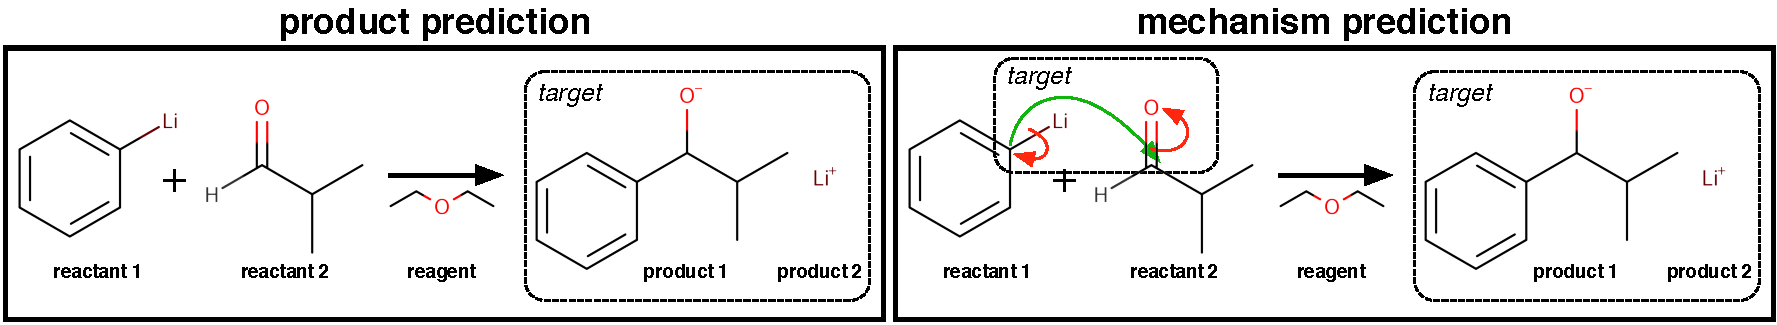
\includegraphics[width=\textwidth]{reaction_diagram.pdf}
\caption{\emph{(Left)} The reaction product prediction problem: Given the reactants and reagents, predict the structure of the product. \emph{(Right)} The reaction mechanism prediction problem: Given the reactants and reagents, predict how the reaction occurred to form the products.}
\label{fig:task-overview}

\end{figure*}

In this section, we begin with a chemistry background on molecules and chemical reactions. We then describe related work in machine learning on predicting chemical reactions. We then describe a particularly important subclass of chemical reactions, called \emph{linear electron flow (LEF)} reactions. Finally, we describe the contributions of this work.



\subsection{Molecules and Chemical reactions.}
Organic (carbon-based) molecules can be represented via a graph structure, where each node is an atom and each edge is a covalent bond (see example molecules in Figure~\ref{fig:task-overview}).
Each edge (bond) represents two electrons that are shared between the atoms that the bond connects. 

Electrons are particularly important for describing how molecules react with other molecules to produce new ones. All chemical reactions involve the stepwise movement of electrons along the atoms in a set of reactant molecules. 
This movement causes the formation and breaking of chemical bonds that changes the reactants into a new set of product molecules \citep{herges1994coarctate}. For example, Figure~\ref{fig:task-overview} (\emph{Right}) shows how electron movement can break bonds (red arrows) and make new bonds (green arrows) to produce a new set of product molecules.

\subsection{Related work}
In general, work in machine learning on reaction prediction can be divided into two categories: 1. \emph{Product prediction}: where the goal is to predict the reaction products, given a set of reactants and reagents, shown in Figure~\ref{fig:task-overview} (\emph{Left}). 2. \emph{Mechanism prediction}: where the goal is to determine {\em how} the reactants react, i.e., the movement of electrons, shown in Figure~\ref{fig:task-overview} (\emph{Right}).


\paragraph{Product prediction.}
% wei2016neural
% NOTE: Jennifer, David and Alan were not the first to apply deep learning to this problem, this was done Aires de Sousa's group already in 2005, using unsupervised pretraining.
Recently, methods combining machine learning and template-based molecular rewriting rules have been proposed [\cite{coley2017prediction,neural-symbolic,segler2018planning,wei2016neural,zhang2005structure}]. Here, a learned model is used to predict which rewrite rule to apply to convert one molecule into another. While these models are readily interpretable, they tend be brittle. 
%The earliest work we are aware of that uses deep learning to predict the products of reactions is \cite{zhang2005structure}. Their idea was to approximate the operations of a molecular fingerprint so that all operations become continuously differentiable. They then learned parameters of this fingerprint to accurately predict product fingerprints end-to-end.
% jin2017predicting
Another approach, introduced by \cite{jin2017predicting}, constructs a neural network based on the Weisfeiler-Lehman algorithm for testing graph isomorphism. They use this algorithm (called WLDN) to select atoms that will be involved in a reaction. They then enumerate all chemically-valid bond changes involving these atoms and learn a separate network to rank the resulting potential products. This method while leveraging new techniques for deep learning on graphs, cannot be trained end-to-end because of the enumeration steps which ensures chemical validity.
% schwaller2017found
\cite{schwaller2017found} represents reactants as SMILES (CITE) strings and then used a sequence to sequence network (specifically, the work of (CITE)) to predict product SMILES. While this method is end-to-end trainable the SMILES representation is quite brittle as often single character changes will not correspond to a valid molecule. The above two methods are state-of-the-art on product prediction and have been shown to outperform the above template-based techniques \citet{jin2017predicting}. Thus we compare directly with these two methods in this work.

% segler2017modelling
% TODO
% segler2018planning
% TODO

\paragraph{Mechanism prediction.}
The only other works we are aware of to use machine learning to predict reaction mechanisms are \cite{fooshee2018deep,kayala2012reactionpredictor,NIPS2011_4356,kayala2011learning}. All of these model a chemical reaction as an interaction between atoms as electron donors and as electron acceptors. They predict the reaction mechanism via two independent models: one that identifies these likely electron sources and sinks, and another that ranks all combinations of them.
These works are complementary to ours as they require expert-curated training sets, for which organic chemists have to hand-code every electron pushing step. %, and is thus designed for small-scale well-known textbook reactions. 
This is in contrast to our work which aims to learn reactions from noisy large-scale reaction datasets. As the above methods cannot use such datasets, we cannot compare directly against them, and we leave a detailed discussion of the pros and cons of each method for future work.
%we leave a detailed comparison of the pros and cons of both methods for future work.
 % (unfortunately the data used to train these models is not currently open-source). 
%However, 
%this combining and then ranking of electron sources and sinks can be a slow process, as many plausible reactions need to be considered \emph{for each electron movement} (the number of subgraphs of $n$ reacting atoms, where single bonds are either added or removed is $2^{n(n-1)/2}$). Furthermore, 
%these models rely on expert-curated training sets, for which organic chemists have to hand-code every electron pushing step (unfortunately the data used to train these models is not currently open-source). As such, this work is complimentary to ours
%These models also have only so far been successfully trained on small hand-curated datasets.
% kayala NIPS: NIPS2011_4356
% kayala2011learning
% kayala2012reactionpredictor
% fooshee2018deep

As a whole, this related work points to at least two main desirable characteristics for reaction prediction models: 
\begin{enumerate}
\item \emph{End-to-End}: There are many complex chemical constraints that limit the space of all possible reactions. How can we differentiate through a model subject to these constraints?
%\item \emph{Graph-Based}: Recent successes in deep learning models for graphs can embed similar graphs to similar vectors. How can we use such models to predict graphs?
\item \emph{Mechanistic}: Learning the mechanism offers a number of benefits over learning the products directly including: interpretability (if the reaction failed, what electron step went wrong), sparsity (electron steps only involve a handful of atoms), and generalization (unseen reactions also follow a set of electron steps).
\end{enumerate}

%In general, a model that predicts the reaction mechanism has a number of benefits over predicting the product of reaction directly: (a) \textbf{interpretability}: If the model makes a mistake, it is easy to see where, and possibly why, it goes wrong by comparing the steps of the mechanism with the correct steps. (b) \textbf{sparse}: Reactions often only affect between 3 and 7 atoms out of anywhere from 10-50 reactant atoms. Modeling the reaction as a path allows one to exploit this sparsity. (c) \textbf{chemically constrained}: Learning a path allows one to easily incorporate chemical constraints, such as the alternating removal and addition of bonds, among others. (d) \textbf{generalizable}: As reaction paths follow similar trends in different molecules, mechanistic models naturally generalize to unseen molecules. 



% We argue that there are a number of benefits of predicting electron paths over predicting the outcomes of reactions directly (as is done in previous work \cite{jin2017predicting,schwaller2017found}):
% \begin{itemize}
% \item \textbf{Easy to interpret}: If the model makes a mistake, it is easy to see where, and possibly why, it goes wrong by comparing the steps of the path with the correct steps.
% \item \textbf{Sparse}: Reactions often only affect between 3 and 7 atoms out of anywhere from 10-50 reactant atoms. Modeling the reaction as a path allows us to exploit this sparsity.
% \item \textbf{Chemically consistent}: Learning a path allows us to easily incorporate chemical constraints, such as the alternating removal and addition of bonds, among others. 
% \item \textbf{Generalizable}: As reaction paths follow similar trends in different molecules, our model naturally generalizes to unseen molecules. 
% \end{itemize}

 



%\begin{wrapfigure}{R}{0.75\textwidth}
%\scriptsize{
%\vspace{-4ex}
%\begin{minipage}{0.75\textwidth}
\begin{table*}[t]
\begin{tabular}{lccc} 
\toprule
 \textbf{Prior Work} & \textbf{end-to-end}  & \textbf{mechanistic} &  \\ %\hline \hline
\midrule
Templates+ML & $-$  & $-$   \\ 
%\cite{coley2017prediction} & $-$ & $-$ & $-$ \\ \hline
WLDN [\cite{jin2017predicting}] &$-$ & $-$  \\ 
Seq2Seq [\cite{schwaller2017found}] & \checkmark & $-$  \\ 
%\cite{segler2017modelling} & \checkmark & $-$ & $-$ \\ \hline 
%\cite{segler2018planning} & \checkmark & \checkmark & $-$  \\ \hline
%\cite{NIPS2011_4356} &$-$ & $-$ & \checkmark  \\ \hline
%\cite{kayala2011learning} & $-$ & $-$ & \checkmark \\ \hline
%\cite{kayala2012reactionpredictor} &$-$ & $-$ &\checkmark  \\ \hline
Source/Sink (expert-curated data) & $-$ & \checkmark \\ 
\midrule
\textbf{this work} & \checkmark  & \checkmark \\
\bottomrule
%\bf{Method} & %\multicolumn{2}{c}{\bf Full} & \multicolumn{2}{c}{\bf Unaware} & \multicolumn{2}{c}{\bf Fair L2} & \multicolumn{2}{c}{\bf Fair L3} \\
\end{tabular}
\centering
	\caption{Work on machine learning for reaction prediction, and whether they are (a) end-to-end trainable, and (b) predict the reaction mechanism. \label{table.existing}}
\end{table*}
%\end{minipage}
%\vspace{-4ex}
%}
%\end{wrapfigure}


Table~\ref{table.existing} describes how the current work on reaction prediction satisfies these characteristics. In this work we propose to model a subset of reactions with \emph{linear electron flow} (LEF), described below.

\subsection{Linear Electron Flow reactions} 
%
Reaction mechanisms can be classified by the topology of their ``electron-pushing arrows'' (the red and green arrows in Figure~\ref{fig:task-overview}). Here, the class of reactions with \emph{linear electron flow} (LEF) topology is by far the most important, followed by those with cyclic topology \citep{herges1994coarctate}. In this work, we will only consider LEF reactions that are \emph{heterolytic}, i.e., they involve pairs of electrons.

If reactions fall into this class, then a chemical reaction can be modeled as pairs of electrons moving in a \emph{single path} through the reactant atoms. 
Further, this electron path will alternately remove existing bonds in molecules, and form new ones. We show this alternating structure in Figure \ref{fig:task-overview} (\emph{Right}). 
The reaction formally starts by (step 1) taking the pair of electrons between the Li and C atoms and moving them to the C atom; this is a remove bond step. 
Next (step 2) a bond is added when electrons are moved from the C atom in reactant 1 to a C atom in reactant 2.
Then (step 3) a pair of electrons are removed between the C and O atoms and moved to the O atom, giving rise to the products. 
Predicting the final product is thus a byproduct of predicting this series of electron steps.


\paragraph{Contributions.} We propose a novel generative model for modeling the reaction mechanism of LEF reactions. Our contributions are as follows
\begin{itemize}
\item We propose an end-to-end generative model for predicting reaction mechanisms, \ourModelR, that is fully differentiable. It can modularly be used with any deep model on graphs.
\item We design a technique to identify LEF reactions and their underlying mechanisms from purely atom-mapped reactants and products, the primary format of large-scale reaction sets.
\item We show that \ourModelR learns untaught chemistry such as functional group selectivity.
\end{itemize}








\section{Model}

\label{sec:model}
% !TEX root =  ../main.tex

\section{Model}



\begin{figure*}
\centering
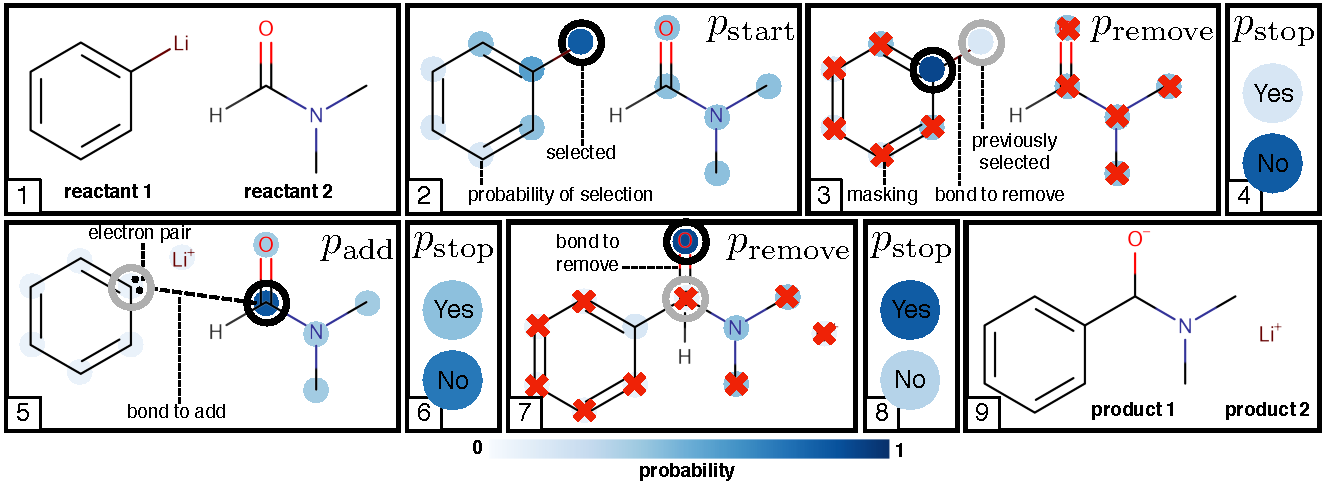
\includegraphics[width=\textwidth]{reaction_model_blue}
\caption{A visualization of the actions taken by the model to sequentially perform a simple reaction.}
\label{fig:reaction_model}
\end{figure*}



In this section we define a probabilistic model that describes the flow of movement of electrons that define an elementary heterolytic reaction.
We represent a set of molecules as a set of graphs $\moleculeSet$, with atoms $\Ac$ as vertices and bonds $\Bc$ as edges;
each connected component of the graph defines an individual molecule.
We can associate an ordering over all the atoms in all the molecules in the set using an {\em atom map} number,
an integer label assigned to each non-hydrogen atom in both the reactants and the products which 
both permits easy matching between atoms before and after the reaction, and
%\footnote{In the USPTO dataset, all reactions have been ``atom mapped'', which means that integer labels have been assigned to each non-hydrogen atom in both the reactants and the products.}. 
gives us a consistent way to index particular atoms.
Each atom $v \in \Ac$ includes a set of features, such as its atom type (e.g. carbon, oxygen, \dots); the full list of input atom features can be found in Table 1 of the supplementary material.
Input molecules into the model are first put in a Kekul\'e form, a process which makes explicit the location of single and double bonds in aromatic structures;
each bond $b \in \Bc$ is either a single, double, or triple bond.


Given an initial set of reactant molecules $\moleculeSet_0$ and a set of reagent molecules $\moleculeSet_r$, 
our model defines a conditional distribution over a sequence of atoms $\electronPath_{0:T} = (a_0, a_1, \ldots, a_T)$,
which fully characterizes the electron path.
\improvement[]{maybe instead $\electronPath$ goes up to $T-1$ and $\moleculeSet$ goes up to $T$? then both are length $T$}
This electron path in turn deterministically defines both a final product $\moleculeSet_{T+1}$, 
denoting the outcome of the reaction,
as well as a sequence of intermediate products $\moleculeSet_t$, for $t = 1,\dots,T$,
which correspond to the state of the graph after the first $t$ steps in the subsequence $\electronPath_{0:t} = (a_0, \dots, a_t)$ are applied to the initial $\moleculeSet_0$.


We propose to learn a parameterized distribution $p_\theta( \electronPath_{0:T} \mid \moleculeSet_0, \moleculeSet_r)$ over electron movements. 
We begin by describing the generative process %(i.e., the forward pass) 
of $p_\theta$, and then describe how to train the model parameters.


\subsection{Generative process}

The joint probability of an electron path can be factorized into a product of distributions
defining the probability $p(a_0 \mid \initialAndReactants)$ of the initial state $a_0$ given the reactants and reagents, 
the conditional probability $p(a_t \mid a_{t-1}, \moleculeSet_t, t)$ \todo[]{maybe somehow refer to "bond type" instead of $t$?} of next state $a_t$ given the intermediate products $\moleculeSet_t$ for $t > 0$,
and the probability $p(s_t \mid \moleculeSet_t)$ that the reaction terminates with final product $\moleculeSet_{t}$.

%The distribution over electron paths can be factorized as follows:
%%\begin{align}
%%p_\theta(\electronPath \mid \moleculeSet_0) = p_\theta(s_{0}' \mid \moleculeSet_0) p_\theta(a_{0} \mid \moleculeSet_0) \prod_{t=1}^{T-1} \left( p_\theta(a_{t} \mid a_{t-1}, \Mc_{t-1} ) p_\theta(s_{0}' \mid \moleculeSet_0) \right) p_\theta(a_{T} \mid a_{T}, \Mc_{T-1} ) p_\theta(s_{T} \mid \moleculeSet_T) \nonumber
%%\end{align}
%
%\begin{align*}
%p(\electronPath_{0:T} \mid \initialAndReactants) = &
% \quad 
% p(s_0' \mid \initialAndReactants)
% p(a_0 \mid \initialAndReactants)
% \prod_{t=1}^{T} \Big[ 
% 	p(s_t' \mid \initialAndReactants, \electronPath_{0:t-1})
% 	p(a_t \mid \initialAndReactants, \electronPath_{0:t-1} ) 
% \Big] \\
% & \times p(s_{T+1} \mid  \initialAndReactants, \electronPath_{0:T} )
%\end{align*}

%\improvement[]{this part a bit messy}
%Where $p(s_{t})$ is the probability of stopping the path before picking the $t^{\text{th}}$ action, $p(s_{t}')$ of continuing.


In practice we assume that the probability of an action depends only on (i) the intermediate molecule formed by the action path up to that point, (ii) the previous action taken (indicating where the free pair of electrons are) and (iii) the point of time through the path, indicating whether we are on an add or remove bond step. 
We further make the simplifying assumption that the stop probability and the actions after $a_0$ do not depend on the reagents. This leads to a parameterized model with dependency structure:
\begin{align}
\label{eq:jointprob}
p_\theta(\electronPath_{0:T} \mid \moleculeSet_0, \moleculeSet_r) 
&=
	p_\theta(s'_0 \mid \moleculeSet_0)
	p_\theta(a_0 \mid \moleculeSet_0, \moleculeSet_r)\\ \nonumber &\quad \times
	\left[\prod_{t=1}^{T}
		p_\theta(s_{t}' \mid \moleculeSet_{t})
		p_\theta(a_t \mid \moleculeSet_{t}, a_{t-1}, t)
	\right]
	p_\theta(s_{T+1} \mid \moleculeSet_{T+1})
	,
\end{align}
where we have defined $p(s'_t \mid \moleculeSet_t) \equiv 1 - p(s_t \mid \moleculeSet_t)$ to be the probability of {\em continuing} a reaction given the current molecule set $\moleculeSet_t$.
%
%
%%% THIS IS THE PREVIOUS VERSION:
%\begin{align*}
%p_\theta(\electronPath_{0:T} \mid \moleculeSet_0, \moleculeSet_r) = &
% \quad \continueProb{0}{0}
%       p(a_0 \mid \moleculeSet_0, \moleculeSet_r)
%       p(a_1 \mid \moleculeSet_0, a_0) \\
%       & \times \prod_{t=2}^{T} \Big[
%              \continueProb{t}{\electronPath_{0:t-1}}
%              \actionProb{t}
%       \Big] \\
%       & \times p(s_{T+1} \mid \moleculeSet_{\electronPath_{0:T}})
%\end{align*}
%
Note that you cannot stop after one action, as you have to pick up a complete electron pair;
however, it is possible to stop prior to selecting a first atom $a_0$, indicating that no reaction would take place.
Given any particular selected atom $a_t$ which extends the reaction path, we can deterministically update the previous molecular graph $\moleculeSet_{t}$ to produce the next set of (intermediate) products $\moleculeSet_{t+1}$.

If the three reaction assumptions stated in the previous section hold, then, as stated earlier, there are two types of electron movements that alternate: 
(1) movement that \emph{removes an existing bond}, and 
(2) movement that \emph{adds a new bond}. 
We can generalize assumption 3 by defining that atoms with free electrons have a self-bond. 
Thus, all reactions start by first selecting an atom, removing a bond (between two different atoms, or a self-bond), and then alternately adding and removing bond;
we can determine whether a particular step is an add step or remove step by inspecting $t$.
Note that $\moleculeSet_1 = \moleculeSet_0$, as the initial action of selecting $a_0$ does not remove or form any bonds\todo{maybe put this somewhere else}.

Each of the conditional probabilities in Eq.~\eqref{eq:jointprob} is parameterized by a neural network:
for each stage the network takes the current intermediate product graph, 
along with the previous action and the reagents if relevant, 
to compute a probability distribution over next possible actions (i.e., selecting a particular atom, or stopping).
These structure of these networks will be described in the following section and more detailed information on the architectures is given in the supplementary material.

Figure~\ref{fig:reaction_model} shows a simple example reaction, which demonstrates all the critical features of the model.
The first subfigure shows two reactants, which we assume will react (i.e.\ $s_0' = 1$).
Subsequent subfigures show the network picking an initial atom to begin the electron path,
and then iteratively selecting atoms for removing and adding bonds, potentially stopping after each action.
Masking at each add and remove step can reduce the total number of possibilities: 
for example, it is not possible to remove a bond which does not exist in the graph $\moleculeSet_t$.
\todo[]{walk through figure. do we want to that HERE, or in the caption? or elsewhere?}

\subsection{Computing atom and molecule features}


We are left now with defining the functional form of our conditional distributions for continuing $p_\theta(s'_t \mid \moleculeSet_t)$, picking the initial action $p_\theta(a_0 \mid \initialAndReactants)$, and picking subsequent actions $p_\theta(a_t \mid a_{t-1}, \moleculeSet_t, t)$.
However, before describing these modules we need to describe how we compute node embeddings and graph embeddings as these  are  essential to each.
Full architectural details (e.g.\ number of layers and hidden units) are deferred to the supplemental material.

Node embeddings are representations of all the atoms (vertices) in all the molecules present in $\moleculeSet_t$.
 We denote them by the matrix $\nodeEmbeddings{\moleculeSet_t} \subseteq \Rc^{|\Ac|\times d}$.
Each row contains a $d$-dimensional embedding of an atom (vertex).
A natural ordering for the rows are  the corresponding atoms' atom-mapped numbers.
We define the function $\fEmbed$ to take in a set of graphs representing each molecule and compute these node embeddings.
In general $\fEmbed$ could be any deep graph model that uses the graph structure of $\Mc_t$ to get graph-isomorphic node features, usually via message-passing techniques \citep{gilmer2017neural};
we choose to use gated graph neural network (GGNN) message functions \citep{li2016gated}.

It is also useful to be able to calculate graph embeddings $\graphEmbeddings$, which are vectors that represent groups of nodes belonging to one or more graphs; i.e.\ an entire molecule or set of molecules.
 We define the function that takes node features belonging to one or more graphs, and calculates their graph embedding by $\fEmbedGraphs$.
These are similar to the readout functions used for regressing on graphs detailed in \citep[Eq. 3]{gilmer2017neural} and the graph embeddings described in \citet[\S B.1]{li2018learning}. \todo[]{check ref the correct parts of these other papers.}
Specifically, $\fEmbedGraphs$ consists of three functions, $\fui$, $\fuj$ and $\fuk$, which could be any MLP but in practice we find that linear functions suffice. % use linear layers for.
There are two stages:
In stage (i), similar to \citet[\S B.1]{li2018learning} we form an embedding of one or more graphs (with vertices $\Ac'$), by performing a gated sum over the node features
\todo{BP: i added $\fuk$ to this equation, so it was all together --- hope this does not cause notational problems elsewhere}
\begin{align}
	\graphEmbeddings = \fuk\big(\sum_{v \in \Ac'} \left[ \mbox{sigmoid}(\fui(\Hb_{\Ac,v})) \cdot \fuj(\Hb_{\Ac,v}) \right]\big).
\end{align}

In this manner the function $\fui$ is used to decide how much that node should contribute towards the embedding,
 and $\fuj$ projects the node embedding up to a higher dimensional space; following \citet[\S B.1]{li2018learning}, we choose to be double the dimension of the node features.
Having formed this embedding of the graphs, we project this down to a lower dimensional space, which is done by the function $\fuk$. 
%Again we use a single linear layer for this function. % already said this above


\subsection{Computing our probabilities over actions}

Having described how we compute node and graph embeddings we are now ready to describe each of our action modules. We start with $p_\theta(s'_t \mid \moleculeSet_t)$, which is the probability of continuing given the set of intermediate products at time $t$. This probability is computed as a graph embedding down to one dimension followed by a sigmoid function: $p_\theta(s'_t \mid \moleculeSet_t) = \sigma(\fEmbedGraphs_{\textrm{stop}}(\nodeEmbeddings{\moleculeSet_t}))$.


This leaves us with describing the form of the initial action, $p_\theta(a_0 \mid \initialAndReactants)$, and picking subsequent actions, $p_\theta(a_t \mid a_{t-1} \moleculeSet_t, t)$, modules.
 The second of these can be broken down into two parameterized functions
$p_\theta^\textrm{remove}(a_t \mid a_{t-1}, \moleculeSet_t)$ for the remove bond step, taken when $t$ is odd, and $p_\theta^\textrm{add}(a_t \mid \moleculeSet_t, a_{t-1})$ for the add bond step, taken when $t$ is even. 
 Each of these three parameterized conditional probability distributions for the {\em initial}, {\em add} and {\em remove} steps have similar forms, and produce a probability vectors over actions as their output. 
 
 Each of these modules start by computing  a single value for each node, so for the initial step we have 
 $\actionLogits_{\textrm{initial}, v} = \fum^\textrm{intial}(\nodeEmbeddings{\moleculeSet_t,v}, \contextVect)$ where $\fum$ is a NN and $\contextVect$ is a context vector. The expressions are similar for the add and remove modules, however with different NNs used for the respective $\fum$ functions.
 Moreover, they also differ in the context vectors, $\contextVect$, which they use; for the add, $p_\theta^\textrm{add}(a_t \mid \moleculeSet_t, t)$, and remove steps, $p_\theta^\textrm{remove}(a_t \mid \moleculeSet_t, t)$, this context vector is the node embedding of the previous action, $\nodeEmbeddings{\moleculeSet_t, a_{t-1}}$. 
 For the initial step, this context vector $\contextVect$ if computed by summing the graph embeddings for each reagent, computed using the embedding function $\fEmbedGraphs_r$.

Finally, each of the modules compute the probability vector over actions. So again starting with the initial step we have 
$p_\theta(a_0 \mid \initialAndReactants) \propto \bm{\beta_\textrm{initial}} \odot \mbox{softmax}(\bm{\actionLogits_{\textrm{initial}}})$, 
with again similar terms for the add and remove steps.  
The $\bm{\beta}$ term is a binary vector, that allows us to mask out specific actions. The value of this differs for the {\em initial}, {\em add} and {\em remove} steps. 
For the initial step any action (or atom) can be picked and so this is 1 everywhere. For the remove step, $\bm{\beta_\textrm{remove}}$ masks out bonds that do not currently exist (although self bonds are allowed in the first step).
For the add step, $\bm{\beta_\textrm{add}}$ only masks out the previous action.



\paragraph{Training}
We can learn the parameters $\theta$ of all the parameterized functions, by maximizing the likelihood of the true path $\log p_\theta(\electronPath_{0:T} \mid \moleculeSet_0, \moleculeSet_r)$.
%\begin{align*}
%%  \min_{\fModules}
%\min_{\theta}
%    & - \log \continueProb{0}{0} - \log p(a_0 \mid \moleculeSet_0, \moleculeSet_r)  - \log p(a_1 \mid \moleculeSet_0, a^*_0) \\
%	& - \sum_{t=2}^{T} \log \Big[ \continueProb{t}{\electronPath_{0:t-1}^*} \actionProb[*]{t} \Big] \\
%    & - \log p(s_{T+1} \mid \moleculeSet_{\electronPath_{0:T}^*})
%\end{align*}
This is evaluated by using a known true electron path $a_t^\star$ and intermediate products $\moleculeSet_t^\star$ extracted from training data,
rather than on simulated values. 
This allows us to train on all stages of the reaction at once.

\paragraph{Sampling}
Once trained we can sample chemically-valid paths from our model using beam search.  This is procedure is described in \todo[]{briefly describe beam search}. 







\section{Reaction Mechanism Identification}

% !TEX root =  ../main.tex

%\subsection{Data and preprocessing}

Our dataset for evaluating our model is a collection of chemical reactions extracted from the US patent database \citep{Lowe2017}.
We take as our starting point the 479,035 reactions, along with the training, validation, and testing splits 
which were used by \citet{jin2017predicting}, referred to as the USPTO dataset.
This data consists of, per reaction, a group of bond changes and reaction SMILES strings \citep{weininger1988smiles}.
The bond changes indicate pairs of atoms which are connected differently in the reactants and products.
The SMILES strings encode the molecules present in a text based format.
Before we can apply our method, we perform two data preprocessing tasks described in the subsections below
(using the open-source chemo-informatics software RDKit \citep{rdkit}).
These steps automatically
extract a subset of data appropriate for training our model of electron movement during a reaction. 


\subsection{Reactant and reagent separation}

Typically, reaction SMILES strings are split into three parts --- reactants, reagents, and products.

The reactant molecules are those which are consumed during the course of the chemical reaction to form the  product, 
while the {\em reagents} are any additional molecules which provide context under which the reaction occurs (for example, catalysts),
but do not explicitly take part in the reaction itself; we see this in the example in Figure~\ref{fig:task-overview}.

Unfortunately, the USPTO dataset as extracted does not differentiate between reagents and reactants.
We elect to preprocess the entire USPTO dataset by separating out the reagents from the reactants using the process outlined in \citet{schwaller2017found}, where we classify as a reagent any molecule for which either 
(i) none of its constituent atoms appear in the product, or 
(ii) the molecule appears in the product SMILES completely unchanged from the pre-reaction SMILES.
This allows us to properly model molecules which are included in the dataset but do not materially contribute to the reaction.

\subsection{Identifying reactions with linear electron topology}

To train our model, it is necessary to extract a ground-truth representation of the electron paths from the SMILES strings and bond changes.
Furthermore, not every reaction in the USPTO dataset has a linear electron topology; 
such reactions (for example, multi-step reactions and cycloadditions) will not have a single unique path through the atoms 
which describes the movement of the electrons.

The first step is to look at the bond changes present in a reaction. 
Each atom on the ends of the path will be involved in exactly one bond change;
the atoms in the middle will be involved in two. 
We can then line up bond change pairs so that neighboring pairs have one atom in common,
 with this ordering forming a path.
For instance, given the pairs "\texttt{11-13, 14-10, 10-13}" we form the unordered path "\texttt{14-10, 10-13, 13-11}".
If we are unable to form such a path, for instance due to two paths being present as a result of multiple reaction stages, then we discard the reaction.

For training our model we want to find the ordering of our path, so that we know in which direction the electrons flow.
To do this we examine the changes of the properties of the atoms at the two ends of our path. 
In particular, we look at changes in charge and attached implicit hydrogen counts. 
The gain of negative charge (or analogously the gain of hydrogen as H$^+$ ions without changing charge) indicates that electrons have arrived at this atom, 
implying that this is the end of the path; 
vice-versa for the start of the path.
However, sometimes the difference is not available in the USPTO data, as unfortunately only major products are recorded, and so details of what happens to some of the reactant molecules' atoms may be missing.
In these cases we fall back to using an element's {\em electronegativity} to estimate the direction of our path, with more electronegative atoms attracting electrons towards them and so being at the end of the path. 

The next step of filtering checks that the path alternates between add steps (+1) and remove steps (-1). 
This is done by analyzing and comparing the bond changes on the path in the reactant and product molecules. 
Reactions that involve greater than one change (for instance going from no bond between two atoms in the reactants to a double bond between the two in the products) can indicate multi-step 
reactions with identical paths, and so are discarded.
Finally, as a last sanity check, we use RDKit to produce all the intermediate and final products induced by our path acting on the reactants,
to confirm that the final product that is produced by our extracted electron path is consistent with the major product SMILES in the USPTO dataset.

The end result of this is extracted reaction paths for those entries in the USPTO dataset which 
correspond to reactions of linear topology.
This comprises $73\%$ of the dataset, containing 349,898 total reactions, of which 29,360 form the held-out test set.





\section{Experiments and Evaluation}
% !TEX root =  ../main.tex

\subsection{Results and Evaluation}

Having trained our model, one surprising challenge is accurately defining what it means for our model to ``correctly'' predict the reaction outcome. 
Part of this relates to whether we are interested in  \emph{Reaction Mechanism Prediction} or \emph{Reaction Product Prediction}. \todo{these should have been described by now using fig 1 but back check.} 
In this section we evaluate our model in each of these regimes in turn.
%Sampling from our model, or selecting high-probability candidates using beam search, yields

\subsubsection*{Reaction Mechanism Prediction}

 For Reaction Mechanism Prediction we are interested in making sure that we got the exact sequence of actions correct.
For instance, when forming a bond between two pairs of atoms we want to know which one of the atoms donated the electron pair needed to form the bond, even if the end result is the same. 

The representation of the reaction mechanism produced by our model is a sequence of atoms, detailing the path taken by the electrons in a series of alternating steps in which bonds are broken and formed; this then can take the form of a sequence of integers.
Here in order to associate a fixed identity with each atom, these integers represent the ``atom mapped'' labels\footnote{In the USPTO dataset, all reactions have been ``atom mapped'', which means that integer labels have been assigned to each non-hydrogen atom in both the reactants and the products.} associated to each atom in the sequence.

The most straightforward approach then to evaluate our accuracy at predicting reaction mechanisms is to check whether the sequence of integers extracted from the raw data (by comparing the reported major product with the reactants\todo[]{change bracket content to "as described earlier"...?}) is an exact match with the sequence of integers output by our \ourModel; the top-1, top-2, top-3, and top-5 accuracies evaluated in this manner are reported in Table \ref{table:mech-predict}.

\begin{table}[h]
  \caption{Results when using \ourModel  for Reaction Mechanism Prediction. Here we count a prediction as correct if the atom mapped action sequences predicted by our model match exactly those extracted from the USPTO dataset.}
  \label{table:mech-predict}
  \centering
  \begin{tabular}{lllll}
    \toprule
    & \multicolumn{4}{c}{Accuracies (\%)}                   \\
    \cmidrule(r){2-5}
    Model Name & Top-1 & Top-2 & Top-3 & Top-5 \\
    \midrule
    \ourModelIR &  70.3 &  82.8 & 87.7 & 92.2    \\
    \ourModelR  &  77.8 &  89.2 & 92.4 & 94.7    \\
    \bottomrule
  \end{tabular}
\end{table}




\subsubsection*{Reaction Product Prediction}

Reaction Mechanism Prediction is useful for ensuring that we formed the correct product in the {\em correct way}.
However, this can underestimate the actual predictive accuracy of the model: 
although a single atom mapping is provided as part of the USPTO dataset, in general atom mappings are not unique; 
when a reactant contains some symmetries, then multiple different atom mappings are effectively equivalent.
Here this would manifest as multiple different sequences of integers which correspond to chemically identical electron paths. An example of a reaction falling under this category is given in the supplementary material.
\sout{An extreme example is a reaction in which one reactant is benzene, a molecule which is formed of six carbon atoms in a completely symmetric ring: while this would be present with a unique atom mapping in the dataset, any reaction path which includes one of these carbon atoms could equally well have selected any of the other five \todo{maybe toss in an inline figure with an example}.}

Recent machine learning approaches to Reaction Product Prediction \citep{jin2017predicting,schwaller2017found}
have evaluated whether the major product reported in the test dataset matches predicted candidate products generated by their system, independent of mechanism.
In our case, the top-5 accuracy for a particular reaction may include multiple different electron paths that ultimately yield the same product molecule.

Identifying whether two product molecules are chemically the same is equivalent to solving a graph isomorphism over the atoms and bond types, comparing the output of our system to the product molecule.
To perform this comparison, we consider an electron path as a sequence of edits performed on the reactants graph, apply these edits to define a product graph, 
and then define a deterministic mapping from the edited graph to a canonical string representation.
This is done by first Kekulizing the molecule, a process which makes explicit the location of single and double bonds in aromatic structures.
We then apply the sequence of edits to the reactants graph,
set explicit charges or hydrogen counts on the first and last atom in the electron path in order to satisfy valence constraints,
and strip all atom map numbers from the graph.
If this graph corresponds to a valid product molecule, we can then use RDKit to express the molecule in a canonical SMILES string format;
predicted electron paths which would yield chemically infeasible products are represented as an empty string.
We can then evaluate whether a predicted electron path matches the ground truth electron path by a string comparison.

To use our model to produce a ranked list of predicted products, we can compute the estimated canonicalized product SMILES for each of the outputs of our beam search over electron paths, removing duplicates along the way. 
These product-level accuracies are reported in \highlight{ROW OF TABLE}.

A benefit of our approach, even if the ultimate the desired goal is to predict the product molecule rather than the electron path,
is that the predicted electron paths then can serve as explanation.
For each predicted product molecule, there is at least one electron path generated by our model which produced this;
whichever of these was highest-ranked by the beam search corresponds to the maximum likelihood path, 
but we can also report the other candidate paths which would produce the sample output as alternative explanations.
\highlight{MAYBE EXAMPLE IN APPENDIX FIGURE.}






% !TEX root =  ../main.tex

\begin{figure*}[t]

    \centering
    \begin{subfigure}[b]{0.3\textwidth}
        \centering
        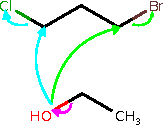
\includegraphics[height=0.9in]{imgs/textbook/reaction3}\\\vspace{0.1in}
        %\caption{}
    \end{subfigure}%
    \hspace{1cm}
     \begin{subfigure}[b]{0.5\textwidth}
        \centering
        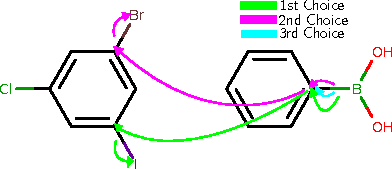
\includegraphics[height=1.1in]{imgs/textbook/reaction7}
        %\caption{}
    \end{subfigure}
%    \vspace{-1em}
	\caption{(Left) 2nd-order nucleophilic substitutions $S_N 2$-reactions, (right) Suzuki-coupling (please note that in the ``real'' mechanism of the Suzuki coupling, the reaction would proceed via oxidative insertion, transmetallation and reductive elimination at a Palladium catalyst. As these mechanistic details are unavailable, we treat Palladium as a reagent). 
    In both cases, our model has correctly picked up the trend that halides lower in the period table usually react preferably ($I>Br>Cl$). }
	\label{fig:qualitative}
\vspace{-0.5em}
\end{figure*}



\subsection{Qualitative Analysis}

Complex molecules often feature several potentially reactive functional groups $\mathcal{F}=\{F_1,...,F_N\}$, which compete for reaction partners. 
To predict the selectivity, that is which functional group will predominantly react in the presence of other groups, 
students of chemistry learn heuristics and trends, 
which have been established over the course of three centuries of experimental observation.
To qualitatively study whether the model has learned such trends from data we queried the model with several typical text book examples from the chemical curriculum (see Figure \ref{fig:qualitative} and the appendix). 
We found that the model predicts most examples correctly. In the few incorrect cases, interpreting the model's output reveals that the model made chemically plausible predictions.




\section{Discussion}


In this paper we proposed \ourModel, a model for predicting electron paths for reactions with linear electron flow.
These electron paths, or {\em reaction mechanisms} provide a detailed description of how molecules react together. 
Our model (i) produces output that is easy for chemists to interpret, and (ii) is able to exploit the sparsity and compositionality involved in chemical reactions, in which often only small numbers of atoms in the reactants interact.
As a byproduct of predicting reaction mechanisms we are also able to perform reaction product prediction,
 and achieve state-of-the-art performance on this task. 
 Work to extend the model towards all classes of chemical reactions is currently ongoing and will be reported in due course.
%
% \paragraph{Acknowledgements.}
%
%
%
%
%We would like to thank Jennifer Wei, Dennis Sheberla, and David Duvenaud for their very helpful discussions.
%BP and MK are supported by The Alan Turing Institute under the EPSRC grant EP/N510129/1. 
%JB acknowledges support from an EPSRC studentship.




%\newpage
\bibliography{bibliography}
%\bibliographystyle{naturemag}
\bibliographystyle{plainnat}

\appendix
\vfill
\pagebreak
\section{Example of symmetry affecting evaluation of electron paths}
In the main text we described the challenges of how to evaluate our model, as different electron paths can form the same products, for instance due to symmetry.
Figure \ref{fig:symmetric-reaction-example} is an example of this.


\begin{figure*}[h]

    \centering
    \begin{subfigure}[b]{0.95\textwidth}
        \centering
        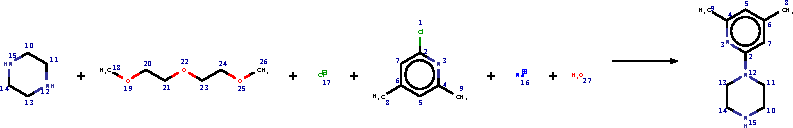
\includegraphics[width=\textwidth]{imgs/symmetry/main_reaction}
        \caption{Reaction as defined by USPTO SMILES}
    \end{subfigure}
    
    \par\bigskip % force a bit of vertical whitespace 
    \begin{subfigure}[b]{0.95\textwidth}
        \centering
        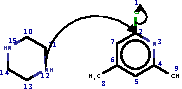
\includegraphics[width=0.4\textwidth]{imgs/symmetry/possible1}
        \qquad
        \qquad
        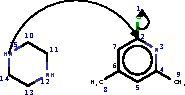
\includegraphics[width=0.4\textwidth]{imgs/symmetry/possible2}
        \caption{Possible action sequences that all result in same major product.}
    \end{subfigure}
    \caption{This example shows how symmetry can affect the evaluation of electron paths. In this example, although one electron path is given in the USPTO dataset, the initial N that reacts could be either 15 or 12, with no difference in the final product. This is why judging purely based on electron path accuracy can sometimes be misleading.}
    \label{fig:symmetric-reaction-example}
\end{figure*}


\section{More training details}

In this section we go through more specific model architecture details omitted from the main text. 

\subsection{Model architectures}
In this section we provide further details of our model architectures.

Section 3 of the main paper discusses our model.
In particular we are interested in computing three conditional probability terms: (1) $p_\theta(a_0 \mid \initialAndReactants)$, the probability of the initial state $a_0$ given the reactants and reagents; 
(2) the conditional probability $p_\theta(a_t \mid \moleculeSet_t, a_{t-1}, t)$ 
%\todo[]{maybe somehow refer to "bond type" instead of $t$?} 
of next state $a_t$ given the intermediate products $\moleculeSet_t$ for $t > 0$;
and (3) the probability $p_\theta(s_t \mid \moleculeSet_t)$ that the reaction terminates with final product $\moleculeSet_{t}$.

Each of these is parametrized by NNs. We can split up the components of these NNs into a series of modules, all introduced in the main text: $\fEmbed$, $\fEmbedGraphs_{\textrm{stop}}$, $\fEmbedGraphs_\mathrm{reagent}$, $\fAdd$, $\fRemove$ and $\fInitial$.
 In this section we shall go through each of these in turn.

The function $\fEmbed$ computes node embeddings, $\nodeEmbeddings{\moleculeSet_t}$, which are used as input to all the other modules. For this we use Gated Graph Neural Networks (GGNN) \citep{li2016gated, gilmer2017neural}.
 We use 4 propagation steps. 
 The atom features we feed in are detailed in Table \ref{table:atom-features}. These are calculated using RDKit. In total there are 101 features and we maintain this dimensionality in the hidden layers during the propagation steps of the GGNN. Three edge labels are defined: single bonds, double bonds and triple bonds. RDKit is used to Kekulize the reactant molecules. 

\begin{table}
  \caption{Atom features}
  \label{table:atom-features}
  \centering
  \begin{tabular}{ll}
    \toprule
    Feature     & Description      \\
    \midrule
    Atom type & 72 possible elements in total, one hot  \\
    Degree     & One hot (0,   1,   2,   3,   4,   5,   6,   7,  10)  \\
    Explicit Valence     & One hot   (0,   1,   2,   3,   4,   5,   6,   7,   8,  10,  12,  14)    \\
    Hybridization & One hot (SP, SP2, SP3, Other) \\
    H count & integer \\
    Electronegativity & float \\
    Atomic number & integer \\
    Part of an aromatic ring & boolean\\
    \bottomrule
  \end{tabular}
\end{table}

As mentioned in Section 3 of the main paper both $\fEmbedGraphs_{\textrm{stop}}$, $\fEmbedGraphs_\mathrm{reagent}$ consist of three
linear functions. 
For  both, the function $\fui$ is used to decide how much each node should contribute towards the embedding and so projects down to a scalar value.
Again for both, $\fuj$ projects the node embedding up to a higher dimensional space, which we choose to be 202 dimensions. 
This is double the dimension of the node features, and similar to the approach taken by \citet[\S B.1]{li2018learning}.
Finally, $\fuk$ differs between the two modules, as for $\fEmbedGraphs_{\textrm{stop}}$ it projects down to one dimension (to later go through a sigmoid function and compute a stop probability), whereas for  $\fEmbedGraphs_\mathrm{reagent}$, $\fuk$ projects  to a dimensionality of 100 to form the reagent embedding.


The modules for $\fAdd$ and $\fRemove$, that operate on each node to produce a action logit, are both NNs consisting of one hidden layer of 100 units. 
Concatenated onto the node features going into these networks are the node features belonging to the previous atom on the path.



The final function, $\fInitial$, is represented by an NN with hidden layers of 100 units. 
When conditioning on reagents (ie for
 \ourModelR
 )
  the reagent embeddings calculated by $\fReagEmbed$ are concatenated onto the node embeddings and we use two hidden layers for our NN. When ignoring reagents (ie for \ourModelIR) we use one hidden layer for this network. In total \ourModelR has approximately 250,000 parameters and \ourModelIR has approximately 190,000.

\subsection{Training}

We train everything using ADAM \citep{kingma2014adam} and an initial learning rate of 0.0001, which we decay after 5 and 9 epochs by a factor of 0.1. 
We train for a total of 10 epochs.
For training we use reaction minibatch sizes of one, although these can consist of multiple intermediate graphs.









\section{Prediction using our model}

At predict time, as discussed in the main text, we use beam search to find high probable chemically-valid paths from our model. Further details are given in Algorithm~\ref{algo:valid_path}.



\newcommand{\cProbCont}{\texttt{calc\_prob\_continue}}
\newcommand{\cProbAct}{\texttt{calc\_prob\_action}}
\newcommand{\cProbInitial}{\texttt{calc\_prob\_initial}}
\newcommand{\removeFlag}{F_\textrm{remove}}

\newcommand{\outputPool}{\hat{\Pc}}
\newcommand{\cPath}{\rho}
\newcommand{\lProb}{p_{\textrm{path}}}


%\begin{wrapfigure}{R}{0.5\textwidth}
\begin{figure}
\begin{minipage}{1.\textwidth}
\begin{algorithm}[H]
  \caption{Predicting electron paths at test time.}
  {\bf Input:}~~Molecule $\Mc_0$ (consisting of atoms $\Ac$), reagents $\Mc_r$ , beam width $K$, time steps $T^\mathrm{max}$
  
  \begin{algorithmic}[1]
  	% Set up pool of completed paths to sort later
  	\STATE $\outputPool = \{\left( \emptyset, \log (1 - \cProbCont(\Mc_0)) \right) \}$  \COMMENT{This set will store all completed paths.}
  	\STATE $\removeFlag \!=\!1$ \COMMENT{remove flag}
  	
  	% Pick the first action.\\
  	\STATE
	\STATE $\hat{\Bc} = \emptyset$.  \COMMENT{This set will store all possible open paths. Cleared at start of each timestep.}	
	\FORALL{$v \in \Ac$} 
		\STATE $ \cPath = (v)$
		\STATE $ \lProb = \log \cProbCont(\Mc_0) + \log \cProbInitial(v, \moleculeSet_0, \moleculeSet_r)$
		\STATE $\hat{\Bc} = \hat{\Bc} \cup \{\left(\cPath, \lProb \right)\}$
	\ENDFOR
	\STATE  $\Bc_{0} = \texttt{pick\_topK\_actions}(\hat{\Bc})$ \COMMENT{We filter down to the top K most promising actions.}
	
	% Then we evaluate the next stages.
	\STATE
	\FOR{t in $(1, \ldots, T^\mathrm{max})$}
		\STATE $\hat{\Bc} = \emptyset $ 
				
		% We take all the previous top K open paths from the previous step...
		\FORALL{$(\cPath, \lProb) \in \Bc_{t-1}$} 
			
			% We evaluate their stop probability at that point and add these stopped version to the completed pool.
			\STATE $\Mc_\cPath = \texttt{calc\_intermediate\_mol}(\Mc_0, \cPath)$
			\STATE $p_c = \cProbCont(\Mc_\cPath)$
			\STATE $\hat{\Pc} = \hat{\Pc} \cup \{(\cPath, \lProb + \log (1 - p_c))\}$
			
			% We then see what would happen if we continued and picked another action.
			\FORALL{$v \in \Ac$}
				\STATE $\cPath' = \cPath^\frown (v)$ \COMMENT{New proposed path is concatenation of old path with new node.}

				\STATE $v_{t-1} = $ last element of $\cPath$
				\STATE $\hat{\Bc} = \hat{\Bc} \cup \{(\cPath' , \lProb + \log p_c + \log \cProbAct(v, \Mc_\cPath, v_{t-1}, \removeFlag) )\}$
			\ENDFOR
		\ENDFOR
		
		% We next prune down the search space for next iteration to our beam width.
		\STATE  $\Bc_{t} = \texttt{pick\_topK\_actions}(\hat{\Bc})$ 
		
		% We indicate that the next step will be opposite step:
		\STATE $\removeFlag = \removeFlag + 1 \mod 2$. \COMMENT{If on add step change to remove and vice versa.}
	\ENDFOR
	
  % Finally we sort the pool and we are done
  \STATE
  \STATE $\outputPool = \texttt{sort\_on\_prob}(\outputPool)$
  \end{algorithmic}
  {\bf Output:}~~Valid completed paths and their respective probabilities, sorted by the latter, ~$\outputPool$
  \label{algo:valid_path}
\end{algorithm}
\end{minipage}
%\end{wrapfigure}
\end{figure}

\section{Further example of actions proposed by our model}

Figure \ref{fig:extra-textbook-example} shows the model's predictions for the mechanism of how two molecules will react. 

\begin{figure*}[h]
        \centering
        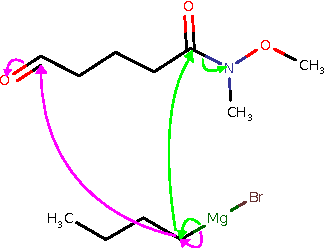
\includegraphics{imgs/textbook/reactants2}
        \caption{Predicted mechanism of our model on reactant molecules. Green arrow shows preferred mechanism, whereas pink shows the model's second preferred choice. Here, the first-choice prediction is incorrect, but chemically reasonable. The second-choice prediction is correct.}
        \label{fig:extra-textbook-example}
\end{figure*}




\end{document}
